% interactcadsample.tex
% v1.03 - April 2017

\documentclass[]{interact}

\usepackage{epstopdf}% To incorporate .eps illustrations using PDFLaTeX, etc.
\usepackage{subfigure}% Support for small, `sub' figures and tables
%\usepackage[nolists,tablesfirst]{endfloat}% To `separate' figures and tables from text if required

\usepackage{natbib}% Citation support using natbib.sty
\bibpunct[, ]{(}{)}{;}{a}{}{,}% Citation support using natbib.sty
\renewcommand\bibfont{\fontsize{10}{12}\selectfont}% Bibliography support using natbib.sty

\theoremstyle{plain}% Theorem-like structures provided by amsthm.sty
\newtheorem{theorem}{Theorem}[section]
\newtheorem{lemma}[theorem]{Lemma}
\newtheorem{corollary}[theorem]{Corollary}
\newtheorem{proposition}[theorem]{Proposition}

\theoremstyle{definition}
\newtheorem{definition}[theorem]{Definition}
\newtheorem{example}[theorem]{Example}

\theoremstyle{remark}
\newtheorem{remark}{Remark}
\newtheorem{notation}{Notation}

% see https://stackoverflow.com/a/47122900

% Pandoc citation processing

\usepackage{hyperref}
\usepackage[utf8]{inputenc}
\def\tightlist{}


\begin{document}

\articletype{ARTICLE TEMPLATE}

\title{An Application of Spatiotemporal Modeling to Finite Population
Abundance Prediction}


\author{\name{Matt Higham$^{a}$, Carly Hammond, John Merickel, Jeff
Wells$^{b}$, add more$^{c, \dagger, \ddagger}$}
\affil{$^{a}$St.~Lawrence University Canton, NY 13617; $^{b}$fill in
later; $^{c}$fill in later}
}

\thanks{CONTACT Matt
Higham. Email: \href{mailto:mhigham@stlawu.edu}{\nolinkurl{mhigham@stlawu.edu}}, Carly
Hammond, John Merickel, Jeff Wells. Email: fill these in later, add
more. Email: \href{mailto:leutnant@fh-muenster.de}{\nolinkurl{leutnant@fh-muenster.de}}}

\maketitle

\begin{abstract}
Insert abstract here.
\end{abstract}

\begin{keywords}
spatial; temporal; kriging;
\end{keywords}

\section{Introduction}

\subsection{Motivation}

Moose surveys in Alaska and western Canada are often performed annually
in many regions. The primary goal of these surveys is to predict moose
abundance, the total number of moose, in the region. Because of time and
money constraints, only some areas (sites) in the region of interest are
selected to be in the survey. Biologists fly to these selected sites,
count the number of moose, and can then use a spatial statistical model
to find a prediction for the finite abundance for that year
\citep{ver2008spatial}.

Though these surveys are annual, each survey is analysed completely
independently of surveys from previous years
\citep[e.g.][]{gasaway1986estimating, kellie_geospatial_2006, boertje2009managing, peters2014contrasting}.
For example, a model for a survey conducted in the year 2019 only uses
counts on sites that were sampled in that year. However, using counts
from previous years in a model that incorporates both spatial and
temporal correlation (spatiotemporal) could result in a prediction for
the realized total or mean that is more precise than predictions from a
spatial model using only counts from the most recent survey year.

Though the framework of the motivation is given with an example on moose
surveys, this type of analysis could be useful for many examples
involving prediction in a finite region with spatial sites that are
surveyed regularly.

\subsection{Background}

\begin{itemize}
\tightlist
\item
  Add paragraph about background of spatiotemporal models
\end{itemize}

Prediction for a total, a subset of the total, or a mean in a finite
number of spatial locations should incorporate a finite population
correction to the variance of the predictor
\citep{ver2008spatial, higham2021adjusting}. In the context of
ecological monitoring in spatiotemporal prediction, we are often most
interested in predicting the total abundance for the most recent year of
the survey. In this case, the finite population correction should adjust
based on the number of sites surveyed in the current year of the survey,
so that, for example, the prediction variance is zero if all sites in
the current year are sampled.

The rest of this paper is organized as follows. In Section
\ref{section:Methods}, we couple spatiotemporal modeling with finite
population prediction to develop the Best-Linear-Unbiased-Predictor for
any linear function of site abundance, including the total abundance
across all sites. In Section \ref{section:Application}, we apply the
predictor to a moose data set in the TOC region of Alaska. In Section
\ref{section:Simulation}, we conduct a brief simulation study to examine
the properties of the predictor. Finally, in Section
\ref{section:Discussion}, we conclude and give directions for future
research.

\section{Methods} \label{section:Methods}

We now give details on the development of the predictor for abundance.
We first detail the spatiotemporal model. Because of the heavy use of
notation in the spatiotemporal model development, we first introduce a
purely spatial model (without temporal variability) and a purely
temporal model (without spatial variability). We then build the
spatiotemporal model and develop a finite population correction factor
to give a Best-Linear-Unbiased-Predictor (BLUP) and its prediction
variance for total abundance in a given year.

\subsection{Spatial Model} \label{subsection:spatialmodel}

First, we consider a spatial linear model for a response variable
\(Y_s(\mathbf{s}_{i})\), \(i = 1, 2, \ldots, n_{s}\), where the vector
\(\mathbf{s}_i\) contains the coordinates for the \(i^{th}\) spatial
site location and \(n_s\) is the number of spatial locations. Then, a
spatial model for \(\mathbf{y}_s(\mathbf{s}_{i})\), a vector of the
\(Y_s(\mathbf{s}_{i})\), is \mbox{} \begin{equation}
\mathbf{y}_s(\mathbf{s}_{i}) = \mathbf{X}_s \bm{\beta}_s + \bm{\epsilon}_s(\mathbf{s}_{i}),
\end{equation}

\noindent where \(\mathbf{X}_s\) is a design matrix for the fixed
effects and \(\bm{\beta}_s\) is a parameter vector of fixed effects. The
error \(\bm{\epsilon}_s(\mathbf{s}_{i})\) can be decomposed into spatial
error and independent error components: \mbox{} \begin{equation}
\label{equation:spatialmodel}
\bm{\epsilon}_s(\mathbf{s}_{i}) = \mathbf{Z}_{s} \bm{\delta} + \mathbf{Z}_{s} \bm{\gamma}.
\end{equation}

\noindent In equation \ref{equation:spatialmodel}, \(\mathbf{Z}_{s}\) is
an \(n_s \times n_s\) matrix of \(0\)'s and \(1\)'s, where the values in
a row corresponding to a data point at location \(\mathbf{s}_{i}\) are a
\(1\) in the \(i^{th}\) column and a \texttt{0} in all other columns.
Note that, without temporal replication, \(\mathbf{Z}_s\) is the
identity matrix so is not necessary to include in equation
\ref{equation:spatialmodel}. \(\bm{\delta}\) is a random vector
independent of \(\bm{\gamma}\) with mean \(\mathbf{0}\) and covariance
\(cov(\bm{\delta}) = \sigma^2_{\delta} \mathbf{R}_{s}\), where
\(\mathbf{R}_s\) is a spatial correlation matrix and
\(\sigma^2_{\delta}\) is sometimes called the spatial partial sill.
\(\bm{\gamma}\) is also a random vector with mean \(\mathbf{0}\) but has
covariance \(cov(\bm{\gamma}) = \sigma^2_{\gamma} \mathbf{I}_{s}\),
where \(\mathbf{I}_s\) is the \(n_s \times n_s\) identity matrix and
\(\sigma^2_{\gamma}\) is sometimes called the spatial nugget.

There are many common parameterizations of \(\mathbf{R}_{s}\). One
common assumption is to assume the covariance function generating
\(\mathbf{R}_s\) is stationary and isotropic, depending only on the
spatial distance between the data points. For example, the exponential
covariance function is defined as follows. For observations at locations
\(i\) and \(i'\) at \(h_{ii'}\) distance apart, row \(i\) and column
\(i'\) of \(\mathbf{R}_{s}\) is equal to \mbox{} \begin{equation}
\label{equation:spatcov}
\text{exp}(-h_{ii'} / \phi),
\end{equation}

\noindent where \(\phi\) is a spatial range parameter controlling the
decay rate of the covariance as distance between two data points
increases.

\subsection{Temporal Model} \label{subsection:temporalmodel}

Next, we consider a temporal linear model for a response variable
\(Y_t(t_j)\), \(j = 1, 2, \ldots, n_{t}\), where the vector \(t_j\)
contains the time for the \(j^{th}\) time point and \(n_t\) is the
number of time points in the data. Then, a temporal model for
\(\mathbf{y}_t(t_j)\), a vector of the \(Y_t(t_j)\), is \mbox{}
\begin{equation}
\mathbf{y}_t(t_j) = \mathbf{X}_t \bm{\beta}_t + \bm{\epsilon}_t(t_j),
\end{equation}

\noindent where \(\mathbf{X}_t\) is a design matrix for the fixed
effects and \(\bm{\beta}_t\) is a parameter vector of fixed effects. The
error \(\bm{\epsilon}_t(t_j)\) can be decomposed into temporal error and
independent error components: \mbox{} \begin{equation}
\label{equation:temporalmodel}
\bm{\epsilon}_t(t_j) = \mathbf{Z}_{t} \bm{\tau} + \mathbf{Z}_{t} \bm{\eta}.
\end{equation}

\noindent In equation \ref{equation:temporalmodel}, \(\mathbf{Z}_{t}\)
is an \(n_t \times n_t\) matrix of \(0\)'s and \(1\)'s, where the values
in a row corresponding to a data point at time point \(t_j\) are a \(1\)
in the \(j^{th}\) column and a \texttt{0} in all other columns. Note
that, without spatial replication, \(\mathbf{Z}_t\) is the identity
matrix so is not necessary to include in equation
\ref{equation:temporalmodel}. \(\bm{\tau}\) is a random vector
independent of \(\bm{\eta}\) with mean \(\mathbf{0}\) and covariance
\(cov(\bm{\tau}) = \sigma^2_{\tau} \mathbf{R}_{t}\), where
\(\mathbf{R}_t\) is a spatial correlation matrix and \(\sigma^2_{\tau}\)
is sometimes called the temporal partial sill. \(\bm{\eta}\) is also a
random vector with mean \(\mathbf{0}\) but has covariance
\(cov(\bm{\eta}) = \sigma^2_{\eta} \mathbf{I}_{t}\), where
\(\mathbf{I}_t\) is the \(n_t \times n_t\) identity matrix and
\(\sigma^2_{\eta}\) is sometimes called the temporal nugget.

There are many common parameterizations of \(\mathbf{R}_{t}\). One
common assumption is to assume the covariance function generating
\(\mathbf{R}_t\) is stationary, depending only on the temporal distance
between the data points. For example, the exponential covariance
function is defined as follows. For observations at time points \(j\)
and \(j'\) at \(m_{jj'}\) units apart, row \(j\) and column \(j'\) of
\(\mathbf{R}_{t}\) is equal to \mbox{} \begin{equation}
\label{equation:tempcov}
\text{exp}(-m_{jj'} / \rho),
\end{equation} \noindent where \(\rho\) is a temporal range parameter
controlling the decay rate of the covariance as time units between two
data points increases. Note that the exponential form of
\(\mathbf{R}_t\) is equivalent to an AR(1) (CITE) time series model if
the time points are equally spaced and the correlation parameter is
greater than zero.

\subsection{Spatiotemporal Model}

We now combine the spatial error components and temporal error
components to formulate a model for data collected across both space and
time. Let \(Y(\mathbf{s}_{i}, t_j)\), \(i = 1, 2, \ldots, n_{s}\) and
\(j = 1, 2, \ldots, n_{t}\), be a random variable, where
\(\mathbf{s}_i\) and \(n_s\) are defined in subsection
\ref{subsection:spatialmodel} and \(t_j\) and \(n_t\) are defined in
subsection \ref{subsection:temporalmodel}. With each spatial location at
each time point, the total number of data points is
\(n_{s} \cdot n_{t} \equiv N\). Then, a spatiotemporal model for
\(\mathbf{y}(\mathbf{s}_{i}, t_j)\), a vector of the
\(Y(\mathbf{s}_{i}, t_j)\), is \mbox{} \begin{equation}
\mathbf{y}(\mathbf{s}_{i}, t_j) = \mathbf{X} \bm{\beta} + \bm{\epsilon}(\mathbf{s}_{i}, t_j),
\end{equation}

\noindent where \(\mathbf{X}\) is a design matrix for the fixed effects
and \(\bm{\beta}\) is a parameter vector of fixed effects. The error
\(\bm{\epsilon}(\mathbf{s}_{i}, t_j)\) can be decomposed into spatial
and temporal components, as in \citet{dumelle2021linear}. Perhaps the
simplest model would be to simply model the error
\(\bm{\epsilon}(\mathbf{s}_{i}, t_j)\) by summing the spatial and
temporal errors defined in equation \ref{equation:spatialmodel} and
equation \ref{equation:temporalmodel}: \mbox{} \begin{equation}
\label{equation:sumcovmodel}
\bm{\epsilon}(\mathbf{s}_{i}, t_j) = \mathbf{Z}_{s} \bm{\delta} + \mathbf{Z}_{s} \bm{\gamma} + \mathbf{Z}_{t} \bm{\tau} + \mathbf{Z}_{t} \bm{\eta}.
\end{equation}

With spatial and temporal replication, \(\mathbf{Z}_s\) is an
\(N \times n_s\) matrix while \(\mathbf{Z}_t\) is an \(N \times n_t\)
matrix. However, even when the spatial covariance function generating
\(\mathbf{Z}_{s} \bm{\delta} + \mathbf{Z}_{s} \bm{\gamma}\) and the
temporal covariance function generating
\(\mathbf{Z}_{t} \bm{\tau} + \mathbf{Z}_{t} \bm{\eta}\) are strictly
positive definite, the sum of the spatial and temporal components is not
necessarily strictly positive definite (\citet{myers1990variograms}).

A more flexible, given in \citet{dumelle2021linear}, is a product-sum
linear mixed model \mbox{} \begin{equation} \label{equation:model}
\mathbf{y}(\mathbf{s}_{i}, t_j) = \mathbf{X} \bm{\beta} + \mathbf{Z}_{s} \bm{\delta} + \mathbf{Z}_{s} \bm{\gamma} + \mathbf{Z}_t \bm{\tau} + \mathbf{Z}_t \bm{\eta} + \bm{\omega} + \bm{\nu},
\end{equation}

\noindent In equation \ref{equation:model}, \(\bm{\omega}\) is a random
vector of length \(N\) with mean \(\mathbf{0}\) and covariance
\(cov(\bm{\omega}) = \sigma^2_{\omega} \mathbf{R}_{st}\) where
\(\mathbf{R}_{st}\) is a spatiotemporal correlation matrix and
\(\sigma^2_{\omega}\) is sometimes called the spatiotemporal partial
sill. \(\bm{\nu}\) is also a random vector of length \(n\) with mean
\(\mathbf{0}\) but has covariance
\(cov(\bm{\nu}) = \sigma^2_{\nu} \mathbf{I}_{st}\), where
\(\mathbf{I}_{st}\) is the \(N \times N\) identity matrix and
\(\sigma^2_{\nu}\) is sometimes called the spatiotemporal nugget.

A common formulation for \(\mathbf{R}_{st}\) is \mbox{}
\begin{equation*}
\mathbf{R}_{st} \equiv \mathbf{Z}_{s} \mathbf{R}_{s} \mathbf{Z}_{s}' \odot \mathbf{Z}_t \mathbf{R}_t \mathbf{Z}_t',
\end{equation*}

\noindent where \(\odot\) is the Hadamard product operator.

If we assume that \(\bm{\delta}\), \(\bm{\gamma}\), \(\bm{\tau}\),
\(\bm{\eta}\), \(\bm{\omega}\), and \(\bm{\nu}\) are mutually
independent of each other, then

\begin{equation}
\label{equation:var}
var(\mathbf{y}) \equiv \bm{\Sigma} = \sigma^2_{\delta} \mathbf{Z}_{s} \mathbf{R}_{s} \mathbf{Z}_{s}' + \sigma^2_{\gamma} \mathbf{Z}_{s} \mathbf{I}_{s} \mathbf{Z}_{s}' + \sigma^2_{\tau} \mathbf{Z}_t \mathbf{R}_t \mathbf{Z}_t'+ \sigma^2_{\eta} \mathbf{Z}_t \mathbf{I}_t \mathbf{Z}_t' + \sigma^2_{\omega} \mathbf{R}_{st} + \sigma^2_{\nu} \mathbf{I}_{st}.
\end{equation}

Note that the model in equation \ref{equation:model} does not have any
distributional assumptions: we only need to specify the mean and
variance of \(\mathbf{y}\). However, if we also assume that
\(\mathbf{y}\) is multivariate normal (with mean
\(\mathbf{X} \bm{\beta} \equiv \bm{\mu}\) and variance \(\bm{\Sigma}\)
(Equation \ref{equation:var})), then all model parameters can be easily
estimated with Maximum Likelihood or Restricted Maximum Likelihood.

\subsection{Finite Population Kriging}

The model in equation \ref{equation:model} is for the \(N\)-length
vector \(\mathbf{y}\). However, often we do not have the resources to
sample or observe every spatial site in every year. Throughout this
section, let the subscript \(o\) denote observations that were observed
(both past and present), the subscript \(u\) denote observations that
were unobserved, and the subscript \(a\) denote all observations. Then,
we can re-order the response vector so that \mbox{} \begin{equation}
\mathbf{y}_a = [\mathbf{y}_u', \mathbf{y}_o']'.
\end{equation}

Let
\(\mathbf{\tilde{y}}_a = [\mathbf{\tilde{y}}_u', \mathbf{\tilde{y}}_o']'\)
denote the fixed, realized values of the response variable for one
data-generating process. Our primary goal is to use the model developed
in equation \ref{equation:model} to predict values for
\(\mathbf{\tilde{y}}_{u}\) from the observed data in
\(\mathbf{\tilde{y}}_{o}\). That is, we want to find optimal weights
\(\mathbf{a}'\) to apply to the observed data
\(\mathbf{a}' \mathbf{\tilde{y}}_o\), such that
\(\mathbf{a}' \mathbf{y}_o\) is the Best Linear Unbiased Predictor
(BLUP) for \(\mathbf{b}_a' \mathbf{y}_a\). For example, if we are
interested in the total abundance across all years, then
\(\mathbf{b}_a\) is a column vector of 1's, so that we are adding up all
values of the response for a predictor of total abundance.

Unbiasedness implies that
\(E(\mathbf{q'}\mathbf{y}_o) = E(\mathbf{b}_a'\mathbf{y}_a)\) for all
\(\bm{\beta}\). So, denoting \(\mathbf{X}_o\) as the design matrix for
sampled sites, \(\mathbf{q'} \mathbf{X}_o \bm{\beta}\) =
\(\mathbf{b'} \mathbf{X} \bm{\beta}\) for every \(\bm{\beta}\), implying
that \(\mathbf{q'} \mathbf{X}_o = \mathbf{b'}_a \mathbf{X}_a\).

The kriging weights are then found by finding \(\bm{\lambda}_s\), an
\(n_o \times 1\) vector, such that \mbox{} \begin{equation}
E\{(\mathbf{q'}\mathbf{y}_o - \mathbf{b'}_a \mathbf{y}_a)(\mathbf{q'}\mathbf{y}_o - \mathbf{b'}_a \mathbf{y}_a)\} - E\{(\bm{\lambda'}_o\mathbf{y}_o - \mathbf{b'}_a \mathbf{z}_a)(\bm{\lambda}_o'\mathbf{y}_o - \mathbf{b'}_a \mathbf{y}_a)\}
\end{equation} \noindent is greater than 0 for all \(\mathbf{q'}\). The
prediction equations are

\begin{equation}
\begin{pmatrix}
\bm{\Sigma}_{o, o} & \mathbf{X}_o \\
\mathbf{X}_o' & 0
\end{pmatrix} 
\begin{pmatrix}
\bm{\lambda} \\
m
\end{pmatrix} = 
\begin{pmatrix}
\bm{\Sigma}_{o, o} & \bm{\Sigma}_{o, u} \\
\mathbf{X}_{o}' & \mathbf{X}_{u}'
\end{pmatrix} 
\begin{pmatrix}
\mathbf{b}_{o} \\
\mathbf{b}_{u}
\end{pmatrix},
\end{equation} \noindent where again the subscripts \(o\) and \(u\)
denote observed and unobserved data points. For example, letting \(n_o\)
denote the number of observed data points, \(\bm{\Sigma}_{o, o}\)
denotes the \(n_o \times n_o\) submatrix of \(\bm{\Sigma}\)
corresponding only to rows and columns of observed data points and
\(\bm{\Sigma}_{u, o}\) denotes the \((N - n_o) \times n_o\) submatrix of
\(\bm{\Sigma}\) corresponding to rows of data points that were not
observed and columns of observations that were observed Then, the
optimal prediction weights \(\bm{\lambda}_o\) are an \(n_o \times 1\)
vector: \mbox{} \begin{equation}
\bm{\lambda}_o' = \mathbf{b}_{o}' + \mathbf{b}_{u}' (\bm{\Sigma}_{u, o}\bm{\Sigma}_{o, o}^{-1}) - \mathbf{b}'_{u}(\bm{\Sigma}_{u, o} \bm{\Sigma}_{o, o}^{-1})\mathbf{X}_o(\mathbf{X}_o'\bm{\Sigma}_{o, o}^{-1}\mathbf{X}_o)^{-1}\mathbf{X}_o'\bm{\Sigma}_{o, o}^{-1} + \mathbf{b}_{u}' \mathbf{X}_{u}'(\mathbf{X}_o'\bm{\Sigma}_{o, o}^{-1}\mathbf{X}_o)^{-1}\mathbf{X}_o \bm{\Sigma}_{o, o}^{-1}.
\end{equation} \noindent Then, the BLUP for
\(\mathbf{b}'_a \mathbf{y}_a\) is \mbox{} \begin{equation}
\hat{\mathbf{b}'_a \mathbf{y}_a} = \bm{\lambda}_o' \mathbf{\tilde{y}}_o,
\end{equation} \noindent with a prediction variance of \mbox{}
\begin{equation}
E((\bm{\lambda}_o'\mathbf{y}_o - \mathbf{b}_a'\mathbf{y}_a)(\bm{\lambda}_o'\mathbf{y}_o - \mathbf{b}_a'\mathbf{y}_a)) = \\
\bm{\lambda}_o'\bm{\Sigma}_{o, o}\bm{\lambda}_o - 2 \mathbf{b}_a' \bm{\Sigma}_{a, o} \bm{\lambda}_o + \mathbf{b}_a' \bm{\Sigma}_{a, a} \mathbf{b}_a.
\end{equation}

A common prediction of interest is the total abundance in the most
recent time point of the survey. Then, \(\mathbf{b}_a\) is a vector of
1's and 0's, where the \(k^{th}\) element of \(\mathbf{b}_a\) is a \(1\)
if the \(k^{th}\) element of \(\mathbf{y}_a\) is from the most current
time point of the survey and the \(k^{th}\) element of \(\mathbf{b}_a\)
is a 0 otherwise. If we order \(\mathbf{y}_a\) with the unobserved, past
data points first, the unobserved, current data points second, the
observed, past data points third, and the observed, current data points
fourth, then \mbox{} \begin{equation}
\mathbf{b}_a = [\mathbf{b}_{up}^\prime, \mathbf{b}_{uc}', \mathbf{b}_{op}', , \mathbf{b}_{oc}']' = [\mathbf{0}', \mathbf{1}', \mathbf{0}', \mathbf{1}']',
\end{equation} \noindent where the subscripts \(up\), \(uc\), \(op\),
and \(oc\) denote unobserved sites in past years, unobserved sites in
current years, observed sites in past years, and observed sites in
current years, respectively.

\(\bm{\lambda}_o\) can then be rewritten as \mbox{} \begin{equation}
\bm{\lambda}_o' = \mathbf{b}_{o}' + \mathbf{b}_{uc}' (\bm{\Sigma}_{uc, o}\bm{\Sigma}_{o, o}^{-1}) - \mathbf{b}'_{uc}(\bm{\Sigma}_{uc, o} \bm{\Sigma}_{o, o}^{-1})\mathbf{X}_o(\mathbf{X}_o'\bm{\Sigma}_{o, o}^{-1}\mathbf{X}_o)^{-1}\mathbf{X}_o'\bm{\Sigma}_{o, o}^{-1} + \mathbf{b}_{uc}' \mathbf{X}_{uc}'(\mathbf{X}_o'\bm{\Sigma}_{o, o}^{-1}\mathbf{X}_o)^{-1}\mathbf{X}_o \bm{\Sigma}_{o, o}^{-1}.
\end{equation}

with a prediction variance of \mbox{} \begin{equation}
\bm{\lambda}_o'\bm{\Sigma}_{o, o}\bm{\lambda}_o - 2 \mathbf{b}_{c}' \bm{\Sigma}_{c, o} \bm{\lambda}_o + \mathbf{b}_{c}' \bm{\Sigma}_{c, c} \mathbf{b}_{c},
\end{equation} \noindent where \(c\) denotes observations in the most
current time point.

\section{Application} \label{section:Application}

\subsection{Data Description}

\begin{figure}
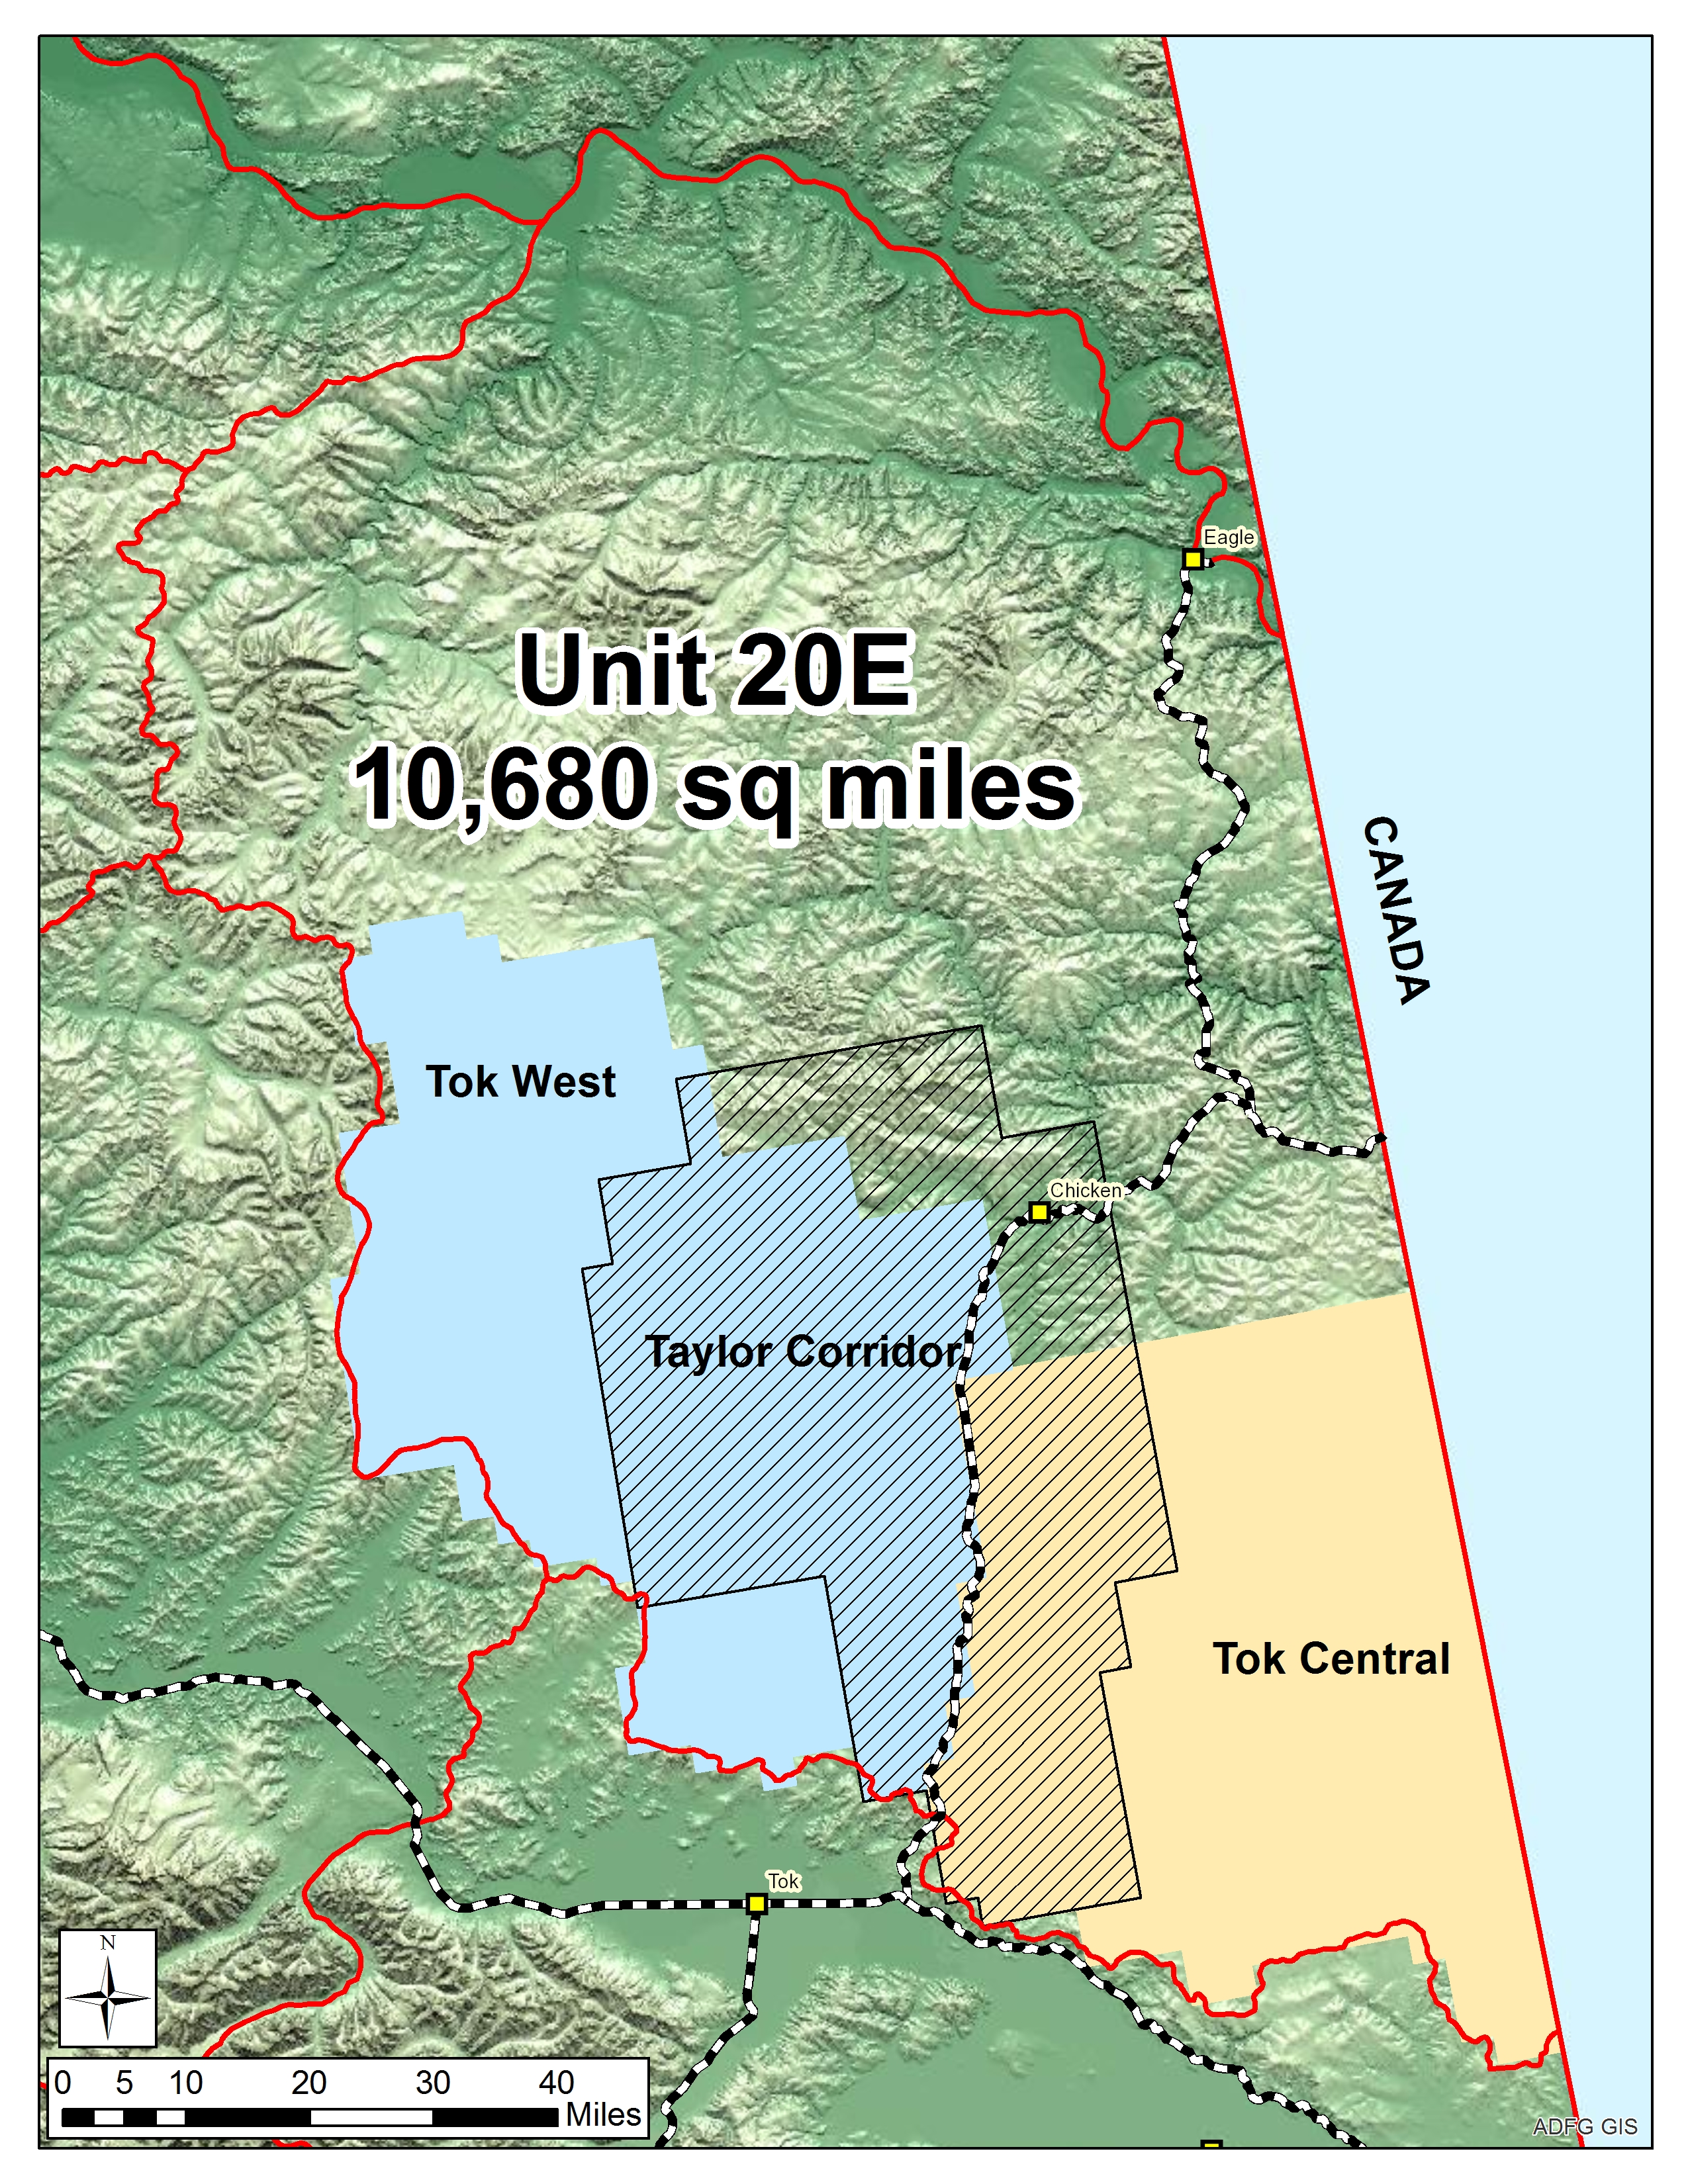
\includegraphics[width=0.5\linewidth]{/Users/highamm/Desktop/FPSpatioTemp/inst/fpspatiotemp_manu/20E_survey_area_overview} \caption{\label{fig:tokplot} A map of the Taylor Corridor in the TOK region of Alaska.}\label{fig:tokplot}
\end{figure}

Abundance surveys are performed in the Taylor Corridor of the TOK region
of Alaska annually (Figure \ref{fig:tokplot}. In particular, surveys
were conducted every year from 2014 through 2020, except for the year
2016, during which there was not sufficient snow cover to perform a
survey. There are a total of 381 unique spatial locations, which we
refer to as ``sites'', and a total of 7 unique time points in the data
set, including the missing year of 2016.

In each year of the survey, an aerial team of biologists selects some of
the 381 sites to survey. The number of sites in the sampling frame that
are selected varies from a low of 76 in the year 2019 to a high of 90 in
the year 2020. Throughout the 7 unique time points, some sites are
surveyed as many as four or five different times while others are never
surveyed.

Before each the survey begins in each year, biologists stratify the
sites into a \texttt{"HIGH"} stratum and a \texttt{"LOW"} stratum. There
are 230 sites in the \texttt{"HIGH"} stratum while there are 151 sites
in the \texttt{"LOW"} stratum. A map of the sites in the TOK region is
given in Figure (make figure and put in figure number).

\subsection{Model Fitting}

We fit the product-sum covariance model defined in equation
\ref{equation:model} using REML, with stratum as a covariate in the
design matrix, an exponential spatial correlation structure defined in
\ref{equation:spatcov}, and an exponential temporal correlation
structure defined in \ref{equation:tempcov}. Table \ref{paramest} gives
the estimated parameters from the model fit.

\begin{table}[ht]
\centering
\begin{tabular}{rrrrrrrrr}
  \hline
 & $\hat{\sigma}^2_{\delta}$ & $\hat{\phi}$ & $\hat{\sigma}^2_{\gamma}$ & $\hat{\sigma}^2_{\tau}$ & $\hat{\rho}$ & $\hat{\sigma}^2_{\eta}$ & $\hat{\sigma}^2_{\omega}$ & $\hat{\sigma}^2_{\nu}$ \\ 
  \hline
1 & 16.9 & 13.3 & 3.8 & 0.9 & 6.9 & 0.2 & 30.8 & 24.0 \\ 
   \hline
\end{tabular}
\caption{Table of estimated covariance parameters in the model.} 
\label{paramest}
\end{table}

To help interpret what some of these fitted covariance parameter
estimates mean, we can construct a fitted covariance plot (Figure
\ref{fig:covplot}). Note that the centroids of two sites directly
adjacent to one another are about 4 units apart. So, we see from Figure
@ref(fig:covplot) that the covariance between random response values
from sites that are adjacent is estimated to be about 20 units if the
response values are in the same year. The covariance between random
responses values from adjacent sites is estimated to be about 10 units
if the response values are 6 years apart. As the spatial distance
between two sites increases, the covariance between the response values
decreases to 0. In fact, the model estimates that, no matter what the
time distance is, when two response values are 20 or more units apart,
the covariance is nearly 0 units.

\begin{figure}
\centering
\includegraphics{fpspatiotemp_manu_files/figure-latex/covplot-1.pdf}
\caption{\label{fig:covplot} Estimated covariance from the fitted
parameters in a product-sum model.}
\end{figure}

Moose surveys in the TOC region were historically analyzed without
explicitly using any data from surveys in past years. Therefore, we
compare the spatiotemporal prediction and prediction interval with a
spatial model fit with the \(\texttt{sptotal}\) package using only the
data from the year 2020. The prediction total abundance is 2888 moose
with a 95\% prediction interval of (2306, 3469) moose. We see that the
predictions are somewhat similar, but that, because the strictly spatial
analysis ignores information from past years, the prediction interval
for the spatiotemporal analysis is more narrow.

\section{Simulation} \label{section:Simulation}

\begin{itemize}
\tightlist
\item
  possibly include \texttt{sptotal} (on current year only) and SRS (on
  current year only) as reference comparisons.
\end{itemize}

For a preliminary simulation, we use a grid of 100 spatial sites and 5
time points. The spatiotemporal process is simulated as a sum-with-error
model with an exponential spatial correlation structure and an
exponential temporal correlation structure with the following parameters

The mean is

\begin{itemize}
\tightlist
\item
  \(\beta\) = 10.
\end{itemize}

The spatial parameters are

\begin{itemize}
\tightlist
\item
  \(\sigma^2_{\delta}\) = 0.9,
\item
  \(\sigma^2_{\gamma}\) = 0.1,
\item
  \(\phi\) = 5.
\end{itemize}

The temporal parameters are

\begin{itemize}
\tightlist
\item
  \(\sigma^2_{\tau}\) = 0.7,
\item
  \(\sigma^2_{\eta}\) = 0.3,
\item
  \(\rho\) = 0.8.
\end{itemize}

And, the spatiotemporal nugget is

\begin{itemize}
\tightlist
\item
  \(\sigma^2_{\nu}\) = 0.4.
\end{itemize}

The sample size \(n\) is 100 (of the 500 total data points). For 100
iterations, the percentage of 90\% prediction intervals that covered the
true total was 81\%.

There are a few plausible reasons for this low coverage:

\begin{itemize}
\tightlist
\item
  there is something incorrect about the method or code used.
\item
  the sample size is only 100 sites, meaning that, on average, only 20
  sites get selected per year. This small sample size may mean that the
  8 parameters cannot be estimated accurately. I believe that this is
  the actual cause of the lower than nominal coverage and hope to do a
  larger simulation study next.
\item
  only 100 simulations were done.
\end{itemize}

Hampering investigation of this is the fact that the simulations take a
long time to run. The \texttt{stmodel} package will be very helpful for
this, as we can replace the slow code for fitting the spatiotemporal
model with faster code from the package.

\section{Discussion} \label{section:Discussion}

\begin{itemize}
\item
  mention substantial reduction of se in the application (and,
  presumably, the simulations).
\item
  mention normal-based-related limitations
\item
  mention Bayesian approach, and its potential flaws
\item
  mention possible extension to imperfect detection
\item
  mention forecasting potential
\item
  take-home message: monitoring programs that use regularly surveys
  might consider incorporating time into their analysis to improve
  precision of predictors (e.g.~NARS for lake assessments).
\end{itemize}

\bibliographystyle{tfcad}
\bibliography{interactcadsample.bib}




\end{document}
